% -*- coding: utf-8; -*-

\chapter{Introduction}
\begin{itemize}
    \color{red}
    \item What is Reference typing?
    \item What is the main representation (from Pierce)?
    \item What we want to propose studying?
    \item What is our alternative representation?
    \item What are the differences
    \item Why should we formalize an idea?
    \item Which Theorems we want to prove?
    \item Which usabilites can we identify by this formalization?
    \item Is this representation simpler or more complicated to prove?
    \item Is this dissertation meant to be didatic?
    \item How formal explaining our syntax?
    \item Define a a typing judgment?
    %%
    \item Explain Mutable References?
    \item Show studies around semantic of mutable reference and typing relations?
    \item  
\end{itemize}
Coq is a expressive functional programming language used for stating and proving logical assertions and a standard tool for researchers to reason about complex language definitions \cite{Pierce_SF1}
Study the implications of bringing this new semantic.
Can be useful for implementing new target languages
"we wish to construct type systems with soundness proofs
that are machine-checkable in the simplest possible logic.
Bring a simplified typing relation, without a store typing
By changing our term syntax to include the type information on loc a ref terms
% \begin{figure}
% \centering
% 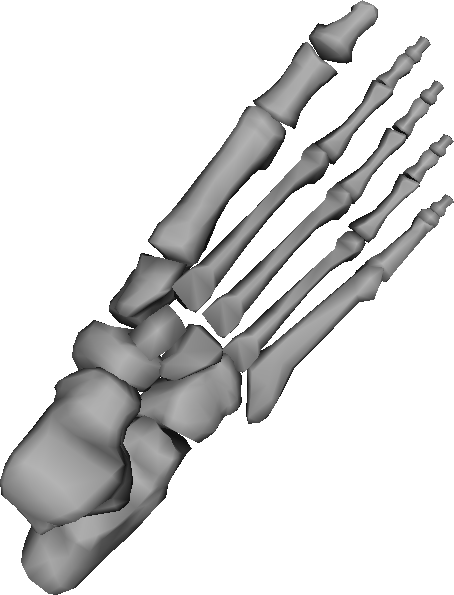
\includegraphics[width=0.45\textwidth]{pictures/image01.png}
% 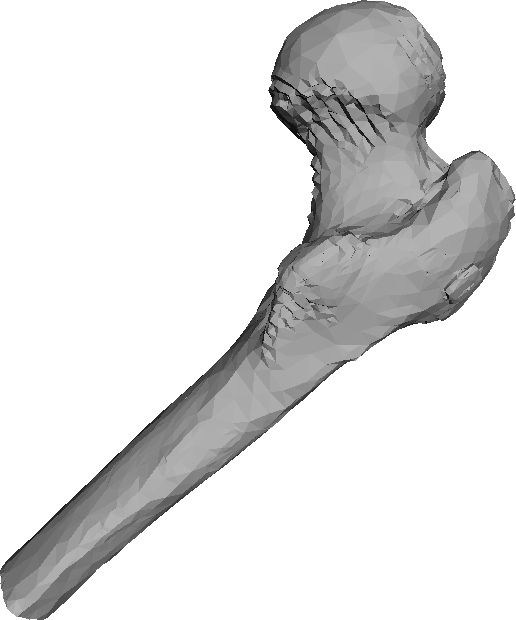
\includegraphics[width=0.45\textwidth]{pictures/image02.png}
% \caption{Meshes generated from medical data. Data obtained from the AIM$@$SHAPE Shape Repository \cite{AIMSHAPE}}
% \label{fig:example}
% \end{figure}


This document is structured as follows. In Chapter~\ref{cha:Previous Work} we present some previous work relevant to our problem. In Chapter~\ref{cha:Proposal} we explain our proposal. In Chapter~\ref{cha:Results} we show our results. Finally, in Chapter~\ref{cha:Conclusion} we present our conclusion and future work.


